\chapter{Research Challenges}
\label{sec:challenges}

\section{Previously Proposed Algorithm}
\label{subsec:kecheng's algorithm}

\noindent
Given a set of microsteps $M$, a set of edges $E$, and a schedule $S$ of a
sequential CCDFG, and pipeline parameters (pipeline
interval $I$ and number of scheduling steps in the loop
$N$), the algorithm~\cite{hrx:dac-12} generates new microsteps, edges and
schedule for the pipelined CCDFG. Values of these inputs are readily available from
intermediate feedback reports from the behavioral synthesis
tool. Given CCDFG $C$, this algorithm replaces
each loop $L$ in $C$ with the pipelined refinement of
$L$. The steps of the algorithm are explained below with the
help of the example introduced earlier in Figure~\ref{fig:high-level-synthesis}(a).

\begin{figure}
\begin{center}
\begin{tabular}{cc}
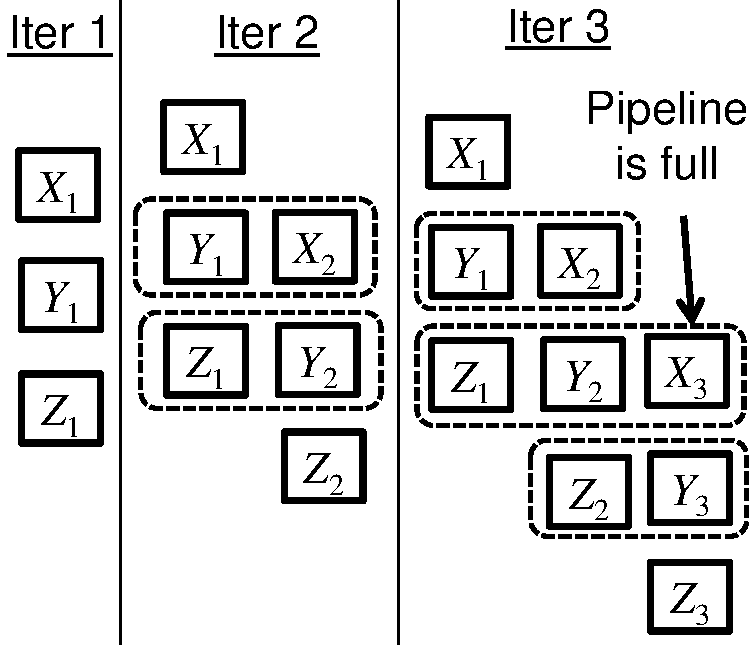
\includegraphics[height=1.7in]{fig-proposal/generate-scheduling-steps}
& %\hspace{0.1cm}
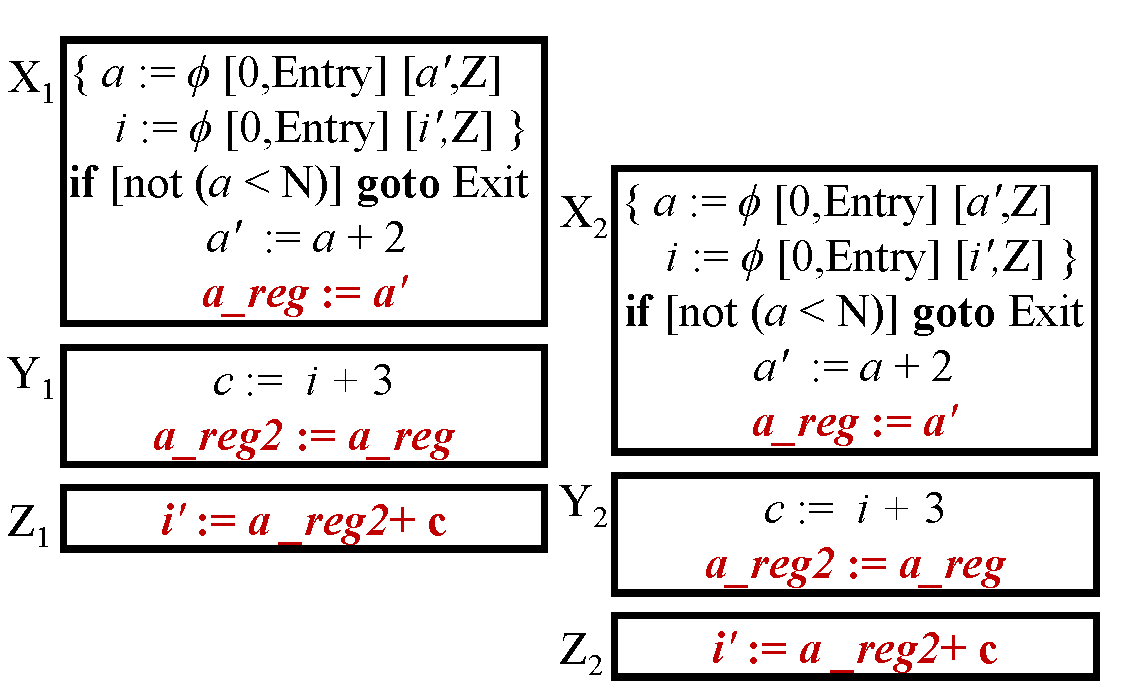
\includegraphics[height=1.7in]{fig-proposal/shadow-reg}
\\
(a) & (b)
\end{tabular}
\end{center}
\caption{(a) Generate scheduling steps. After the pipeline is full, adding new iteration simply repeats the pipeline full stage. (b) Generate shadow registers.}
\label{fig:algorithm}
\end{figure}

%\begin{enumerate}[--]
{\bf Generate scheduling steps:} Figure~\ref{fig:algorithm}(a) shows the addition of scheduling steps of new iterations of a loop according to the pipeline interval. Here, the loop has three scheduling steps and a pipeline interval of one. The new scheduling steps are generated till the pipeline is full. This step generates a new schedule.
For the sake of easily identifying microsteps later, every microstep in the unrolled loop is given a unique name even though
a microstep is the same across different iterations. We would later see how
this trivial step affects the theorem proving process adversely.

{\bf Generate shadow registers:} In order to pipeline a loop, we have to remove data hazards. We first identify all variables that can be overwritten when executing overlapped iterations and then introduce new temporary variables called shadow registers to avoid overwrites. In Figure~\ref{fig:algorithm}(b), the value of $a'$ will be overwritten in $X_2$ before $Z_1$ can read it. So, we introduce a new pipeline register $a\_reg$ which gets assigned the value of $a'$ and replace subsequent reads of $a'$ with reads of $a\_reg$. In the next scheduling step, $a\_reg2$ is assigned the value of $a\_reg$ and further subsequent reads of $a'$ are replaced with reads of $a\_reg2$. Introducing shadow registers in such a way removes the possibility of data hazard as the value of the old variable is stored in a new temporary shadow variable every scheduling step.

\begin{figure}[t!]
\begin{center}
\begin{tabular}{cc}
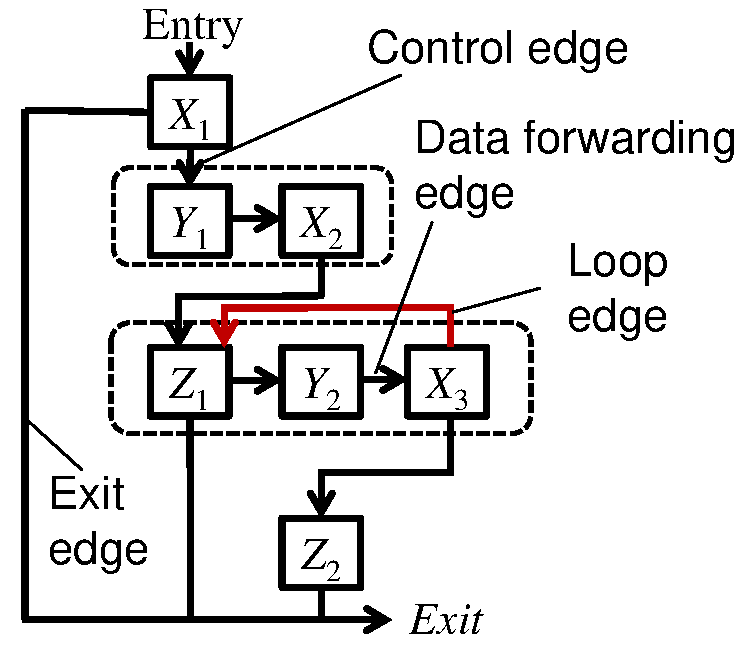
\includegraphics[height=1.6in]{fig-proposal/generate-edges}
& %\hspace{0.1cm}
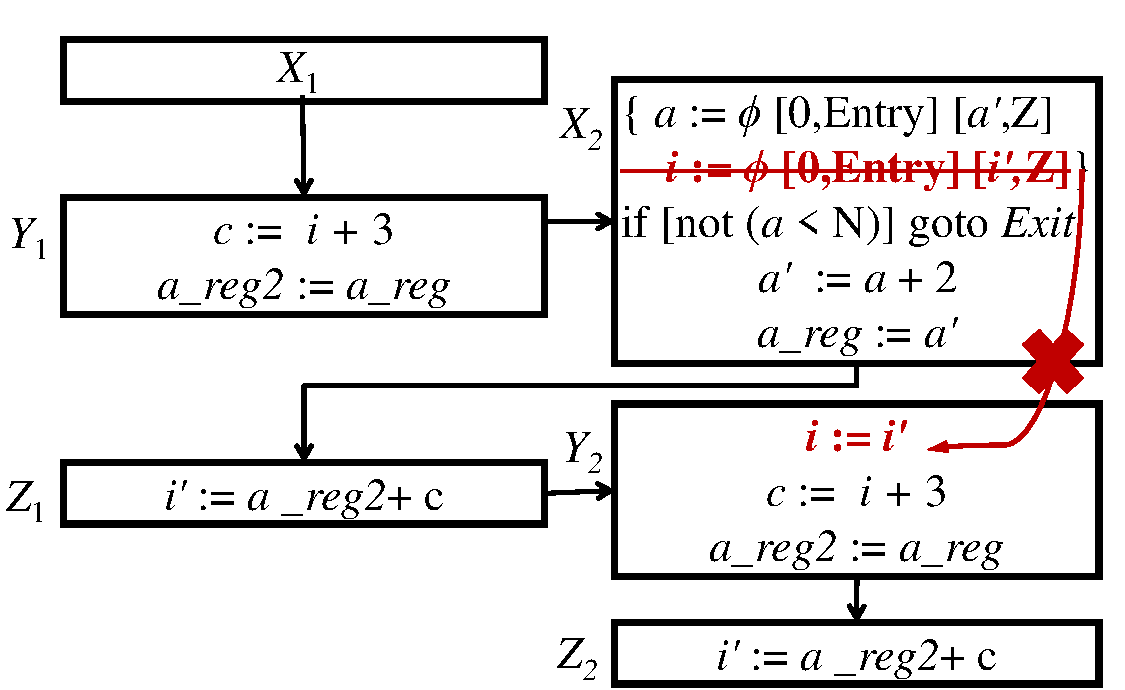
\includegraphics[height=1.6in]{fig-proposal/data-forwarding}
\\
(a) & (b)
\end{tabular}
\end{center}
\caption{(a) Generate edges for pipelined CCDFG (b) Data propagation.}
\label{fig:algorithm-2}
\end{figure}

{\bf Generate edges:} The algorithm adds the edges for data and control flow as shown in Figure~\ref{fig:algorithm-2}(a). Control edges are edges from one scheduling superstep to the next. Data forwarding edges forward data from one scheduling step to the next in a single scheduling superstep. Loop edge denotes the repetition of the pipeline full stage. Exit edges are from the scheduling steps to the $Exit$ block. Note that a pipelinable loop has only one $Exit$ block. Even though the concept of $Exit$ edges was introduced, but they were not implemented in the algorithm.

{\bf Generate data propagation:} In Figure~\ref{fig:algorithm-2}(b), we require the value of $i'$ in $X_2$ to execute the following statement:
$$ i := \phi [0, Entry][i', Z]$$
But, if we execute $X_2$ before executing $Z_1$, the value of $i'$ has not yet been produced. To avoid such a situation, the algorithm relocates the assignment statement $i := i'$ to $Y_2$ just before it needs to be read. The assignment statement $i := i'$ is obtained from the $\phi$-statement $i := \phi [0, Entry][i', Z]$ since in the sequential execution, we would have entered $X_2$ from $Z$ block.

This relocation is however incorrect. Note that we have moved the assignment statement across the conditional branch. $$ if [not (i<N)] goto Exit $$ If we would have executed the sequential CCDFG and the exit condition in the second iteration is true, we would have executed the microstep $i := i'$ before exit. However, now in the pipelined CCDFG, if we exit in $X_2$, we do not execute the microstep $i := i'$. Hence, the value of $i$ is not same in the sequential and pipelined CCDFGs. This is a bug that we found in this algorithm: it incorrectly allows relocation of microsteps across conditional branch statements.
We realized that the authors of the previous proposed algorithm had not accounted for the exit conditions while testing the algorithm. As a result, this bug was not found prior to our formalization. We provide a fix to this bug in our loop pipelining algorithm in Section~\ref{sec:pipelining-algorithm}.

Even after we fix the bug in the proposed algorithm, it is not easy to verify this algorithm as it is.
We elaborate below on the challenges
in verifying the proposed algorithm and in general, any complex algorithm not written while keeping theorem proving in mind.
%\end{enumerate}

\section{Challenges in Verifying Previous Algorithm}

To understand the complexities involved in mechanical
certification of an algorithm that was not designed
originally with certification in mind, we need to re-visit
the general approach to applying formal reasoning on
software programs.  The typical approach is to break the
program into a number of pieces, prove key lemmas
characterizing the role of each piece, and then chain these
lemmas together into a proof of the correctness of the
entire program. Crucial to this approach, however, is the
requirement that each program piece can be characterized by
a succinct invariant that can be easily verified.  However,
in a program not developed with reasoning in mind,
optimizations typically destroy the structural disciplines
and modularity of the individual program pieces. This makes it
difficult to identify and isolate the components that
actually maintain succinct, interesting invariants.

For instance, to prove the correctness statement in the previous algorithm, 
we want to prove that the complete algorithm follows
the invariant that the semantic run of input CCDFG is equal to semantically running the output CCDFG.
Since the algorithm is composed of four concrete steps -- generate scheduling steps, add shadow register,
add edges and data propagation, we intuitively expect the individual steps or at least a combination of steps in sequence to
follow this invariant. However, since the algorithm has not been designed keeping theorem proving
in mind, that is not the case. For example, if
we consider the first step of the proposed algorithm -- {\bf generating new scheduling steps} by
overlapping executions of an unrolled loop, we know that the semantic run 
of the sequential scheduling steps is not the same as the run of new scheduling steps
unless we prove that there are no data hazards. But, data hazards are not completely eliminated till the last step of the algorithm. Note, that the complete algorithm
does follow the invariant as expected, but reasoning about the structure of the
complete algorithm at once is not easy.

In addition, the previous algorithm does not take a CCDFG as input, but rather
works with microsteps, edges and schedule of a CCDFG. That can get tricky because to analyze the
semantic run of a CCDFG, we have to now simultaneously analyze all the three inputs. In our approach,
we work with the CCDFG itself and define the run of a CCDFG semantically.

Furthermore, the previous algorithm initially unrolls the loop and later adds
a back edge to mimick the pipeline full stage. Unrolling loop with unique names
for each microstep makes it easier to design the algorithm but formally we lose the notion
that each microstep is part of a loop and not different in each iteration.
Besides, unrolling loop makes it very difficult to reason for the correctness of the
back edge in the
full pipeline stage.

In general, in order to certify such an arbitrary implementation,
one has to either (1)~restructure the implementation into
one that is more disciplined, and prove the equivalence
between the two, or (2)~come up with very complex
invariants that essentially comprehend how invariants from
each individual piece are conflated together in the
implementation.  Both approaches require extensive human
interaction, resulting in the proverbial euphemism of proofs
of programs being orders of magnitude more complex than the
programs themselves~\cite{liu}.

In our work, however, we can ``get away'' without verifying
the specific implementation while still being able to
certify the design generated by behavioral synthesis without
loss of fidelity. The key observation, as above, is that it
is sufficient to develop {\em any} certifiable algorithm
that generates a pipelined CCDFG from a sequential
implementation which can be effectively applied with SEC.
In particular, any certifiable algorithm that has the same
input-output characteristic as the proposed algorithm
is sufficient.  Thus, this dissertation focuses on identifying
certifiable primitives and invariants of a loop pipelining
transformation and developing a pipeline generation
algorithm using those primitives, achieving the dual goal of
mechanical reasoning of the algorithm and amenability of the
resulting reference model to SEC.

\section{Enhancements: Think about name of section}

Proving an algorithm using mechanical theorem prover gives us the confidence that the pipelined design is indeed correct. We can claim that if a pipeline loop is created, then there are no additional data hazards which have not been accounted for. {\bf rewrite : Also, since our final theorem proves that executing a sequential loop with branches randomly is same as executing a pipelined loop with branches randomly, we can confidently say that data and control flow is well-maintained}.   

Because of the inherent need to make sure that each step of the algorithm maintaines the control flow, we had to deal with branches.  
The previous algorithm introduces the concept of Exit edges but does not explain/implement them. We checked with the authors of the previous algorithm. They checked the output of their algorithm with RTL under the assumption that the loop never exits, hence they did not face any issue while testing. However, removing a conditional branch in a loop and furthermore, adding the conditional branch back in the middle of a pipelined full loop stage requires a complex reasoning which we manage using one of our primitives, explained in ~\ref{sec:pipelining-algo}.

Also, the requirement that data flow is maintained at each step enabled us to find a bug in the previous algorithm. The previous algorithm moves a statement to make sure one particular data hazard is removed, but in doing so they move the statement across a conditional branch statement. Our primitves ensure that such a move is not possible. We have restructred the data propagation step so that instead of going across a conditional branch in the same iteration, the movement of step is now to the previous iteration. 

Furthermore, there is a different mindset required when we merely write an algorithm Vs when we want to prove an algorithm using theorem proving. For example, adding a shadow register step may look like a trivial step which requires reasoning about read and write variables, but when we have to mathematically prove that such a step maintains the control and data flow, we have to reason about the fact that the new variable is indeed a new variable not introduced anywhere else in the algorithm. Moreover, after adding one such variable, the state of original CCDFG is no longer the same as new CCDFG since new shadow variable has been introduced. 


